\documentclass{article}
\usepackage{graphicx}
\usepackage{listings}
\usepackage{color}
\usepackage{float}
\usepackage{tikz}

\title{Practical Work 4: MapReduce Word Count}
\author{Nguyen Thanh Dat \\ Student ID: 23BI14091}
\date{}

\begin{document}

\maketitle

\section{Introduction}
The objective of this practical work is to implement a **Word Count** application using the **MapReduce** programming model. MapReduce is a framework for processing large data sets with a parallel, distributed algorithm on a cluster.

\section{Implementation Choice}
I chose to implement a custom MapReduce framework using **Python and MPI (mpi4py)**. 
\begin{itemize}
    \item \textbf{Why Python:} It provides native dictionary structures (\texttt{defaultdict}) that are perfect for counting unique keys (words).
    \item \textbf{Why MPI:} Since C/C++ frameworks are currently limited, I utilized MPI to "invent" a parallel framework where processes communicate to scatter data and gather results.
\end{itemize}

\section{Mapper and Reducer Design}
The logic follows the standard MapReduce workflow:

\begin{figure}[H]
    \centering
    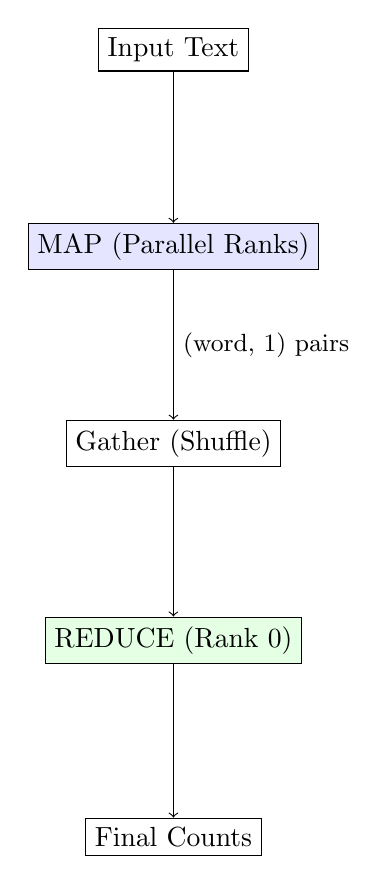
\begin{tikzpicture}[node distance=2.5cm, auto]
        \node (input) [draw, rectangle] {Input Text};
        \node (map) [draw, rectangle, below of=input, fill=blue!10] {MAP (Parallel Ranks)};
        \node (shuffle) [draw, rectangle, below of=map] {Gather (Shuffle)};
        \node (reduce) [draw, rectangle, below of=shuffle, fill=green!10] {REDUCE (Rank 0)};
        \node (output) [draw, rectangle, below of=reduce] {Final Counts};

        \draw[->] (input) -- (map);
        \draw[->] (map) -- node[right]{\small (word, 1) pairs} (shuffle);
        \draw[->] (shuffle) -- (reduce);
        \draw[->] (reduce) -- (output);
    \end{tikzpicture}
    \caption{MapReduce Workflow Architecture}
\end{figure}

\begin{itemize}
    \item \textbf{Mapper:} Each MPI Rank receives a subset of the text lines. It iterates through the words, converting them to lowercase and incrementing a local counter.
    \item \textbf{Reducer:} The "Master" process (Rank 0) gathers the dictionaries from all Ranks and aggregates the values for each unique word.
\end{itemize}

\section{Code Snippet}
\begin{lstlisting}[language=Python, basicstyle=\small, frame=single, breaklines=true]
# Mapper Logic
for word in line.lower().split():
    my_counts[word] += 1

# Reducer Logic
for partial_dict in all_counts:
    for word, count in partial_dict.items():
        final_counts[word] += count
\end{lstlisting}

\end{document}